%%
% The BIThesis Template for Graduate Thesis
%
% Copyright 2020-2023 Yang Yating, BITNP
%
% This work may be distributed and/or modified under the
% conditions of the LaTeX Project Public License, either version 1.3
% of this license or (at your option) any later version.
% The latest version of this license is in
%   https://www.latex-project.org/lppl.txt
% and version 1.3 or later is part of all distributions of LaTeX
% version 2005/12/01 or later.
%
% This work has the LPPL maintenance status `maintained'.
%
% The Current Maintainer of this work is Feng Kaiyu.
%
% Compile with: xelatex -> biber -> xelatex -> xelatex

\chapter{Related Work}
\section{ELF File Structure}

The ELF file format, the abbreviation for Executable and Linkable Format, is a standard binary format that is widely adopted in Unix-like operating systems such as Linux and FreeBSD for describing executable files, object files, shared libraries, and kernel dump files. Because of its superior extensibility and support among different platforms, the ELF format is defined as a core bridge for executing programs and linking libraries in modern operating systems. A typical ELF file primarily contains the following four critical structures:

\begin{enumerate} [label=\arabic*)] 
\item ELF Header

\item Program Header Table

\item Section

\item Section Header Table

\end{enumerate}

\begin{figure}[hbt]
	\centering
	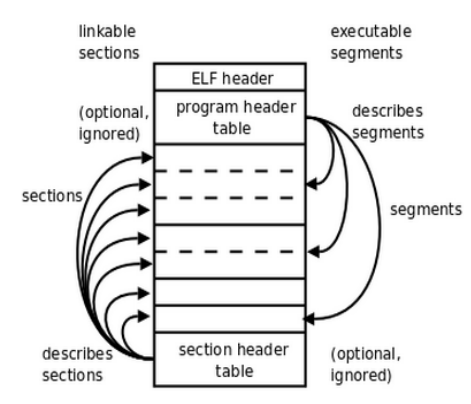
\includegraphics[width=0.75\textwidth]{figures/2.1}
	% \caption[这里的文字将会显示在 listoffigure 中]{这里的文字将会显示在正文中}
	\caption{ELF File Structure}\label{fig:2.1}
\end{figure}

\section{Malware Detection Technologies}

Currently, malware detection technologies are primarily classified into the following three types, which are expressed in Figure \ref{fig:2.2}:

\begin{figure}[hbt]
	\centering
	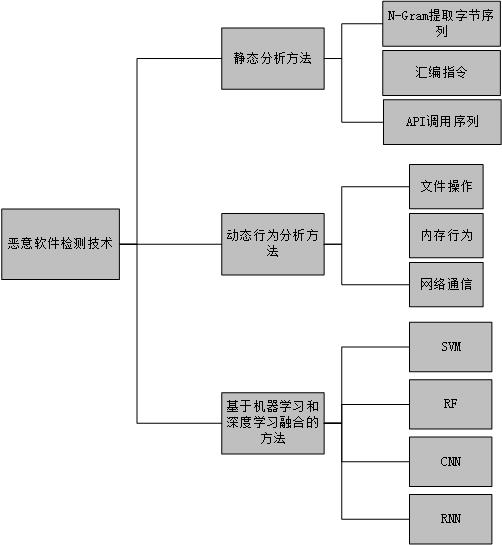
\includegraphics[width=0.75\textwidth]{figures/2.2}
	% \caption[这里的文字将会显示在 listoffigure 中]{这里的文字将会显示在正文中}
	\caption{Malware Detection Methods Classification}\label{fig:2.2}
\end{figure}

 
(1)静态分析方法

Static analysis is the earliest technique used for malicious code detection, which mainly first uses reverse engineering of software binary files to extract static features such as traits, string information, import tables, section structures, instruction sequences, and operation code frequencies, then uses signature matching or machine learning methods to classify and judge. Kumar et al. proved that classifiers based on combining raw and derived values of PE headers and comparing integrated feature sets against original feature sets can detect and classify malware with high accuracy\cite{kumar2019learning}. Yan et al. proposed a novel malware classification system using deep graph convolutional networks to embed control flow graphs (CFGs), validating its effectiveness on two large datasets that contain over 20,000 samples\cite{yan2019classifying}. Corlatescu et al. issued a static analysis-based malware detection framework and constructed the EMBER benchmark dataset based on file structure information and metadata\cite{corlatescu2023embersim}. Ling et al. raised MalGraph, a neural network method relying on hierarchical graph for robust Windows malware detection, capturing executable file interaction and structure semantics through function call graphs and control flow graphs\cite{ling2022malgraph}.

This approach's advantages include high speed and low resource consumption, making it suitable for large-scale sample initial sifting. However, its weaknesses are also obvious, such as lacking the ability to recognize malware processed with packing, obfuscation, and code injection, which can make malware evade easily.

(2)动态行为分析方法

Dynamic analysis executes suspicious programs in virtual sandboxes or controlled environments, monitoring their behaviors which include dynamic features such as system call sequences, file operations, registry modifications, and network communications when they are executed to determine whether the programs are malicious. Trizna et al. proposed Nebula, a self-attention Transformer architecture for dynamic malware analysis\cite{trizna2024nebula}. Through noting, filtering, normalizing, and encoding behavioral reports and adapting Transformer structure, they conducted comprehensive studies to evaluate system component effect on performance. Bhat et al. performed dynamic behavioral analysis on Android applications by system call analyzing, extracting dynamic features to use integrated learning algorithms for classification\cite{bhat2023system}. Li et al. dynamically analyzed software API call sequences in secure virtual environments, transformed these sequences into multiple feature expressions, and using deep learning models including Bi-LSTM to classify them\cite{li2022novel}. Chen et al. proposed an API sequence learning method based on parameter augmentation, which can achieve high detection robustness and generalization ability through deep neural network training\cite{chen2022cruparamer}. Rohini et al. raised MAGIC, which quantifies malware behaviors through behavioral co-occurrence and regression analysis\cite{rohini2024magic}. Experimental results showed MAGIC is more accurate in reflecting signature maliciousness than traditional methods, enhancing malware defense capabilities.

This method focuses more on detecting actual behaviors, which means it is robust against mutation or obfuscated samples. However, it suffers from higher resource consumption and remains vulnerable to being evaded through delayed execution or anti sandbox detection techniques. Furthermore, some highly targeted APT attack samples may not reveal true behaviors in virtual sandboxes, which leads to false negatives.

(3)基于机器学习和深度学习融合的方法

Recently, with the rapid development of artificial intelligence, an increasing number of researchers adopt machine learning and deep learning methods to solve malware detection tasks. By extracting static or dynamic features from samples and training classification models such as Support Vector Machines (SVM), Random Forest (RF), Convolutional Neural Networks (CNN), and Recurrent Neural Networks (RNN), researchers achieved significant detection results on multiple public datasets. Ngo et al. introduced a rapid malware detection method combining static and dynamic features, enhancing detection efficiency via transfer learning\cite{ngo2023fast}. Through deep learning extracting latent characteristics to resolve feature dimension inconsistency problems and knowledge distillation, this method transfers aggregated feature knowledge to static feature models, which can achieve detect more rapidly. Shar et al. extracted 14 features from Android applications, comparing traditional machine learning methods such as random forest and deep learning methods such as recurrent neural networks performance on these features\cite{shar2023experimental}. Bashir et al. extracted static and dynamic features, such as API calls and permission, from Android applications, and classified them by using SVM, K-NN, Naive Bayes, and integrated learning methods\cite{bashir2024hybrid}.

This approach has adaptive capabilities and feature abstraction abilities, but detection results often depend on training data with distributional consistency, which makes it face insufficient robustness against adversarial samples or newly emerging threats.  

\section{Adversarial Malware}

Adversarial malware refers to malicious samples that attackers precisely disturb, with the premise that the original malicious sample functionalities are not broken, causing them to be misrecognized as benign software during detection and then evade detection systems. These disturbances can be implemented at code levels such as instruction insertion and control flow adjustment; at structural levels such as section table modification, symbol table perturbation; or at behavioral levels such as API call sequence pretense with high concealment and targeting specifically.

Unlike static data such as images, malware samples have complex execution semantics and latent behavioral logic. Therefore, generating adversarial samples for malware requires not only guaranteeing structural validity but also ensuring the original sample behaviors' executability. This characteristic makes adversarial sample generation considerably more complex and challenging in the malware realm.

Currently, multiple methods have been proposed for generating adversarial malware, mainly including the following categories:

Methods Based on Gradients: Methods such as FGSM\cite{lupart2023study} (Fast Gradient Sign Method) and PGD\cite{bryniarski2021evading} (Projected Gradient Descent) regard samples as vectors and calculates model gradients to find disturbance directions that are most likely to cause misclassification. However, these methods are mostly suitable for continuous spaces like images, and their effectiveness is limited when processing discrete structures in executable files.


Methods Based on Heuristics and Searches: These methods model disturbance operations as search problems and utilize genetic algorithms\cite{wang2022black}, simulated annealing\cite{bertsimas1993simulated}, Monte Carlo tree search\cite{chaslot2010monte}, and other similar techniques to find optimal disturbance paths with executability constraints. Their advantage is high customizability, but a balance often happens between search efficiency and sample quality.

Methods Based on Reinforcement Learning: Recently, Reinforcement Learning has gradually become a hotspot in adversarial sample generation research because of its advantages in policy learning. Attackers build an agent that learns a sequence of disturbance strategies to evade detection systems and uses evasion rate as a reward target. Common methods including Q-learning\cite{watkins1992q}, DQN\cite{osband2016deep}, and PPO \cite{yu2022surprising}(Proximal Policy Optimization) can achieve adaptive disturbance policy learning and optimization while ensuring sample legitimacy.

\section{Reinforcement Learning}

Reinforcement Learning (RL) is an artificial intelligence learning method based on trial-and-error mechanism. Its core principle is that an agent continuously adjusts its strategy through interactions with the environment to get maximize long-term returns, guided by reward signals. Different from supervised learning, Reinforcement Learning does not rely on definite label information but learns the value of behaviors through environmental feedback. It exhibits strong adaptability and online learning capabilities, which makes it widely applicable to tasks such as game strategy optimization, robotic control, natural language processing, and adversarial sample generation.

\begin{figure}[hbt]
	\centering
	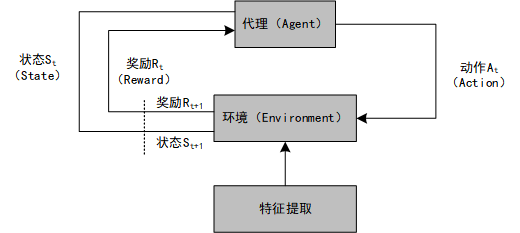
\includegraphics[width=0.75\textwidth]{figures/2.3}
	% \caption[这里的文字将会显示在 listoffigure 中]{这里的文字将会显示在正文中}
	\caption{Markov Decision Process}\label{fig:2.3}
\end{figure}

The target of Reinforcement Learning is to learn an optimal policy $\pi^{*}(a|s)$ that maximizes the expected cumulative reward which is defined as the sum of discounted rewards at each future moment starting from the current moment $t$:
\begin{equation}
	\label{eq:reward}
	\boldsymbol{G}_t = \sum_{k=0}^{\infty} \gamma^k r_{t+k}
\end{equation}

In this formulation,\( r_{t+k} \) is the reward obtained from Step \( k \) starting from time \( t \), and \( \gamma^k \) represents the discount factor of Step \( k \).

\section{Neural Networks and Sequential Modeling Techniques}

Neural Networks (NNs) are computational models simulating the structure and executing functionality of the human brain, widely applied in image recognition, natural language processing, and intelligent decision-making. Their basic architecture includes an input layer, one or more hidden layers, and an output layer. Each layer connects to the previous layer's neurons through weights and introduces nonlinear capabilities by using activation functions, enabling the network to approximate complex nonlinear mapping relations.

In the cybersecurity domain, neural networks have been employed for tasks such as malware detection, anomaly behavior recognition, and attack traffic detection, achieving notable results. However, many security tasks have dynamic features such as high temporal dependency, tight contextual linkage, and complex behavioral logic, which cause traditional feedforward neural networks to be struggle to capture these dynamic features effectively.

\subsection{Recurrent Neural Network(RNN)}

Recurrent Neural Networks (RNNs) are specialized neural network models for processing sequential data. Their key feature is their memory capability, enabling them to use the information from previous time steps when processing current inputs. Unlike traditional feedforward networks, RNN hidden layers receive not only current inputs but also previous hidden layers’ outputs, achieving modeling temporal dependencies. This structure makes RNNs particularly suitable for processing sequential data like text, voices, and video frame sequences.

In RNN, each step's computation passes the previous step's state (hidden layer output) to the next step, combining it with current inputs to propagate and accumulate information in sequence. However, during the real training process, RNNs often suffer from gradient vanishing or gradient explosion because gradients require multiple time steps to achieve propagating back during the backpropagation, which makes the model difficult to capture long-term dependencies.

\begin{figure}[hbt]
	\centering
	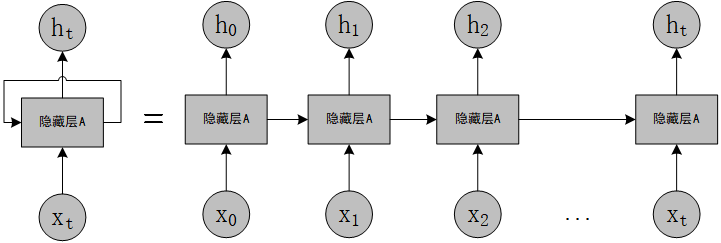
\includegraphics[width=0.75\textwidth]{figures/2.4}
	% \caption[这里的文字将会显示在 listoffigure 中]{这里的文字将会显示在正文中}
	\caption{RNN Neural Network Structure}\label{fig:2.4}
\end{figure}

\subsection{Long Short-Term Memory(LSTM)}

The Long Short-Term Memory (LSTM) \cite{graves2012long} is a special RNN designed to overcome the issue that traditional RNNs suffer from gradient vanishing and gradient explosion when processing long sequences. Unlike common RNNs, LSTM adapts carefully designed "gating mechanisms" to selectively remember or forget information from sequences, thus effectively capturing long-term dependencies. LSTM is widely used in natural language processing, voice recognition, and time-series prediction.

The LSTM core structure contains three gating units: Input Gate, Forget Gate, and Output Gate, along with a Cell State that is used to carry long-term memory information.

Input Gate controls which parts of current input are written into the memory cell.

Forget Gate determines which information from the previous memory state should be retained or forgotten.

Output Gate decides which parts of the current memory state are passed to the next time step as the hidden state.

The key to LSTM is that the cooperation of these three gates enables LSTM to control the information flow precisely, retaining useful information for model predictions while discarding irrelevant or redundant data. Its information flow is described as follows: First, the forget gate decides which old information should be discarded based on current input and previous hidden state; Second, the input gate determines how much new input should be written into the memory cell; Third, the memory state updates; Finally, the output gate generates a hidden state from current memory state for passing to the next time step.

This design can make LSTM continuously retain valid information in long sequences and ignore irrelevant parts, overcoming the disadvantages of traditional RNN in modeling dependency on long-term.


\begin{figure}[hbt]
	\centering
	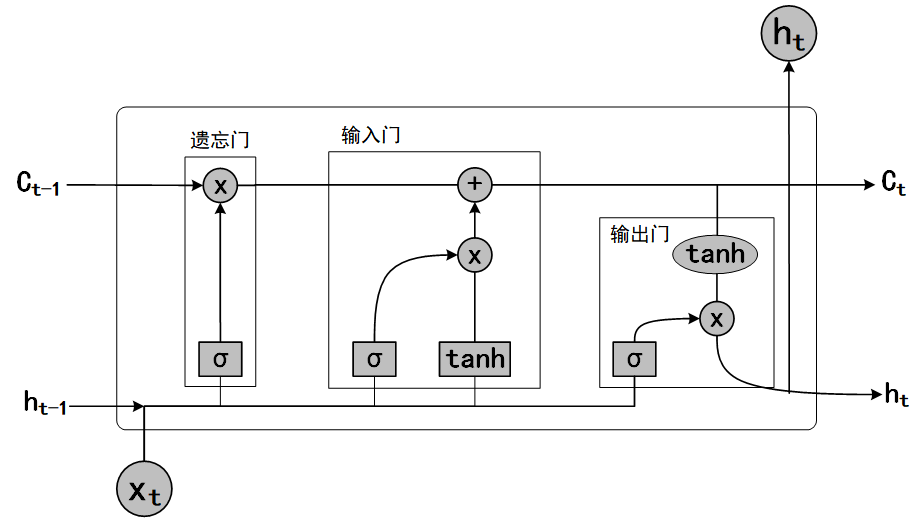
\includegraphics[width=0.75\textwidth]{figures/2.5}
	% \caption[这里的文字将会显示在 listoffigure 中]{这里的文字将会显示在正文中}
	\caption{LSTM Basic Data Cell Structure}\label{fig:2.5}
\end{figure}

Due to malware's behavioral features and disturbance operations having obvious sequential reliance and contextual relation, malware samples generate sequences of API calls, system behaviors, or instruction flows during execution, where contextual information is crucial for identifying malicious actions and implementing effective disturbances. Maintaining long-term dependencies is nearly impossible for traditional fully connected NNs or standard RNNs when processing this sequential data, with frequently forgetting early information in sequences. In contrast, LSTM's gating mechanisms enable gate-controlled mechanisms including Input Gate, Forget Gate, and Output Gate, which can effectively control information retention and forgetting, preserve long-term dependencies and enhance the model's ability to capture disturbance sequence semantics. Generally, while generating disturbance strategies, LSTM can dynamically adjust strategy outputs based on the current sample state and historical disturbance operations, producing samples that are not only more "aggressive" but also modified by highly concealed adversarial disturbances. This memory capability is essential for generating malicious behaviors that exhibit "sequential logic" and can evade detection systems.

\section{PPO}

Proximal Policy Optimization (PPO) is a reinforcement learning algorithm based on policy gradients\cite{yu2022surprising}, introduced by OpenAI in 2017. As an improved version of Trust Region Policy Optimization (TRPO), PPO remains the core stable policy updates concept of TRPO while significantly simplifying the algorithm's implementation and training process. Because of its robustness and efficiency, PPO has become one of the most widely used and consistently stable algorithms in deep reinforcement learning.

The core target of PPO is to limit the magnitude of changes between old and new policies, thus preventing drastic fluctuations during policy updates and ensuring learning process stability. Different from traditional policy gradient methods that directly maximize objectives, PPO introduces a clipped objective function or a penalty term modification based on KL divergence to constrain differences between old and new policies.

In the clipped objective function form, PPO's optimization objective is described as below.
\begin{equation}
	\boldsymbol{r}_t(\theta) = \frac{\boldsymbol{\pi}_\theta(\boldsymbol{a}_t | \boldsymbol{s}_t)}{\boldsymbol{\pi}_{\theta_{\text{old}}}(\boldsymbol{a}_t | \boldsymbol{s}_t)}
\end{equation}

In this equation, \( \boldsymbol{r}_t(\theta) \) is the action probability ratio between the current policy and the old policy. By minimizing this clipped objective function, PPO effectively prevents policy updates from deviating too far from the old policy, enhancing the stability during training process.

\begin{figure}[hbt]
	\centering
	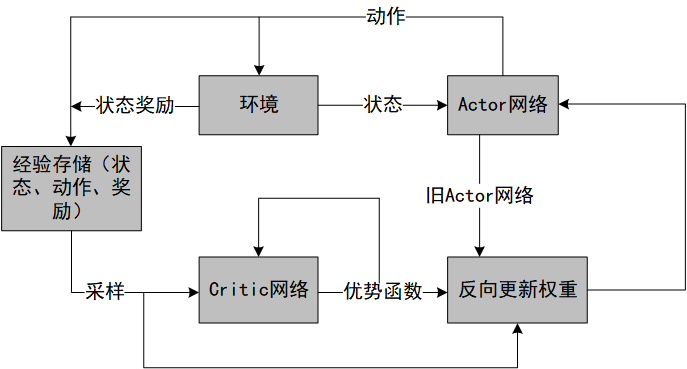
\includegraphics[width=0.75\textwidth]{figures/2.6}
	% \caption[这里的文字将会显示在 listoffigure 中]{这里的文字将会显示在正文中}
	\caption{PPO Refinforcement Learning Model's Structure}\label{fig:2.6}
\end{figure}

